
\section{Our Approach}

The general idea is to apply image analogies using stereoscopic data to generate new stereoscopic data.
We simply present the ideas here and implementation details are provided in the following section.

The general steps are:
\begin{enumerate}
	\item \textbf{Select} patches in stereo database that match our monocular image patches
	\item \textbf{Transfer} the corresponding stereoscopic data to synthesize the output frame from our input frame
	\item On a \textbf{scale pyramid} to work at different levels of detail
\end{enumerate}

\subsection{Selecting patches}
The selection of pixels or patches from the database corresponds to finding the Nearest Neighbor Field (NNF) between the patches of our new image and those of our database.

Brute-force computation is not tractable given the quantity of data we are facing.
We chose to implement the PatchWeb algorithm~\cite{Barnes11} that extends Patch Match~\cite{Barnes09} to multiple exemplar NNF computation.

\subsection{Transfering the stereoscopic data}
Having a candidate patch in our database (with its corresponding right/left frame patch\footnote{Without loss of generality, we assume that our input corresponds to a left frame in our database.}), we propose different transfer strategies, namely transferring: the \emph{whole patch}, the \emph{patch difference}, or the \emph{patch disparity} as illustrated in Figure~\ref{fig:transfers}.

\begin{figure*}[ht!]
	\centering
	\begin{subfigure}[b]{0.29\textwidth}
	\centering
		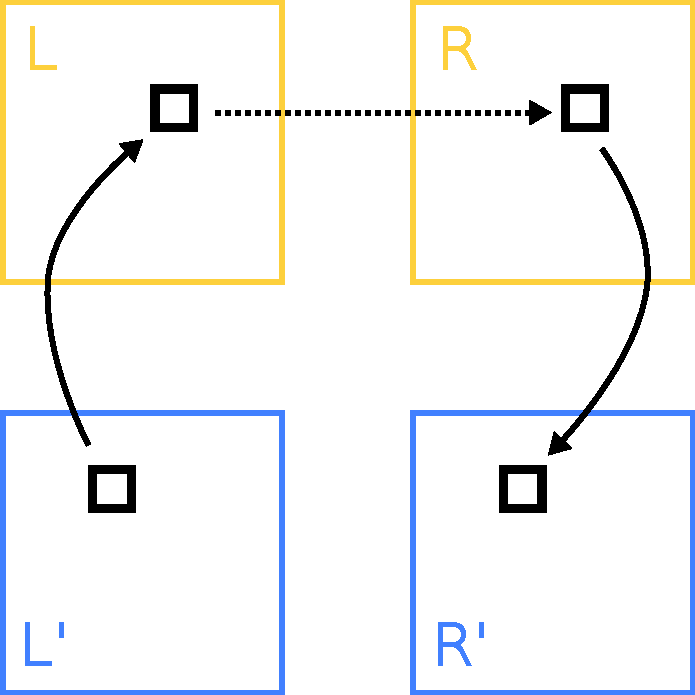
\includegraphics[height=3.6cm]{figures/transfers-A}
		\\
		$L' \to R'=R\phantom{)}$
		\caption{Transferring the whole patch}
	\end{subfigure}
	\begin{subfigure}[b]{0.29\textwidth}
	\centering
		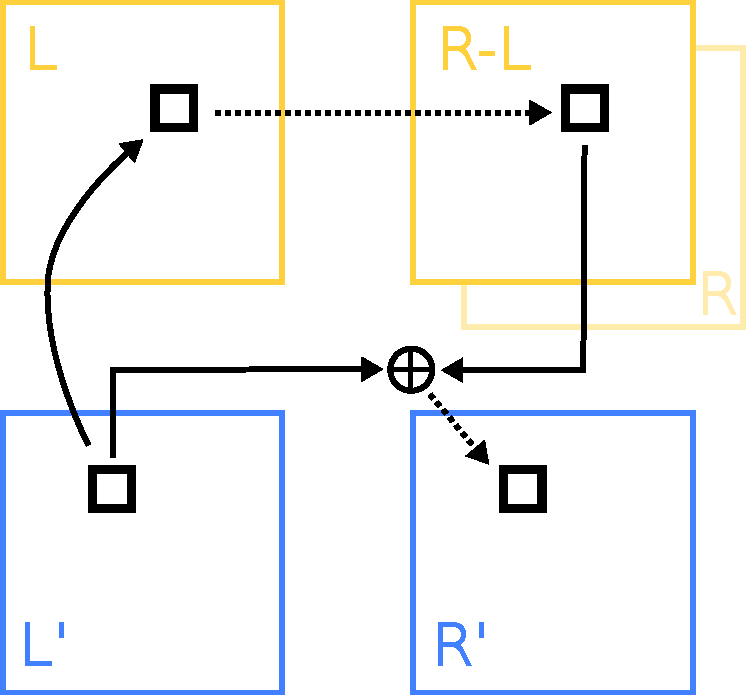
\includegraphics[height=3.6cm]{figures/transfers-B}
		\\
		$L' \to R'=L'+(R-L)$
		\caption{Transferring the patch difference}
	\end{subfigure}
	\begin{subfigure}[b]{0.4\textwidth}
	\centering
		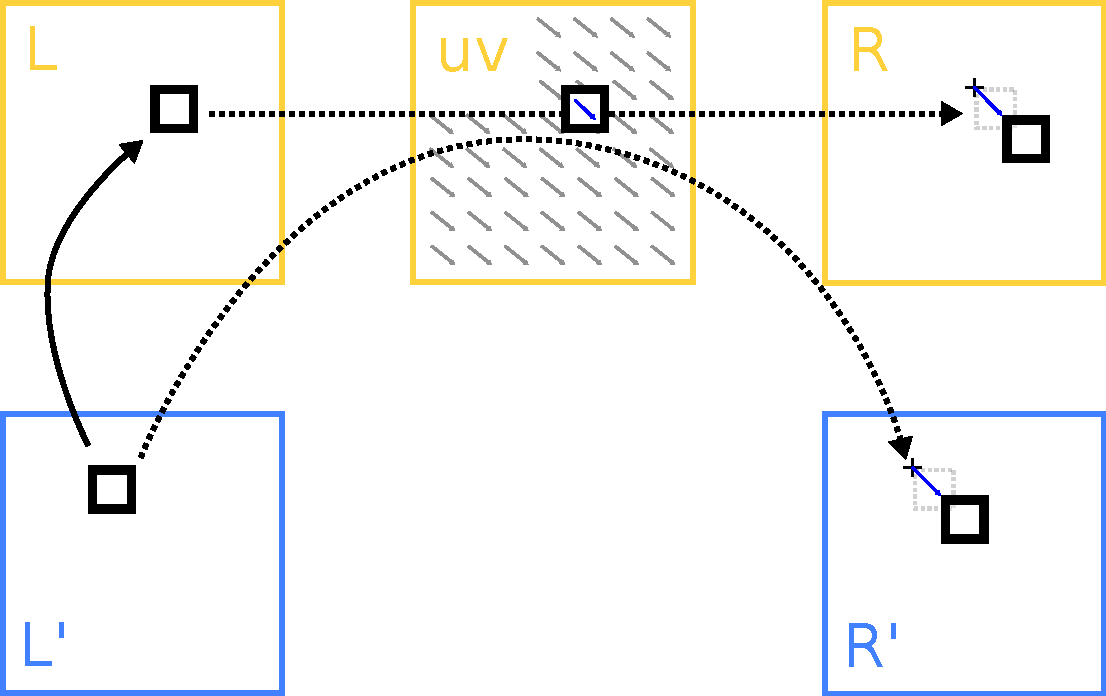
\includegraphics[height=3.6cm]{figures/transfers-C}
		\\
		$L' \to R'=\textrm{warp}_{L\to R}(L')$
		\caption{Transferring the disparity}
	\end{subfigure}
	\caption{Three strategies for stereoscopic data transfer: we synthesize $R'$ from $L'$ given a corresponding mapping $L\to R$}
	\label{fig:transfers}
\end{figure*}

\subsection{Pyramidal processing}
Since different objects and features appear at different scales, we apply the aforementioned selection and transfer on a scale pyramid, in a coarse to fine manner.

